\documentclass[12pt]{article}
\usepackage[utf8]{inputenc}
\usepackage{amsmath}
\usepackage{amsfonts}
\usepackage{amsthm}
\usepackage{amssymb}
\usepackage{alltt}
\usepackage{array}
\usepackage[backend=bibtex,style=ieee,]{biblatex}
\usepackage{blindtext}
\usepackage{bold-extra}
\usepackage{caption}
\usepackage{copyrightbox}
\usepackage{dirtree}
\usepackage{enumitem}
\usepackage{float}
\usepackage[margin=25mm]{geometry}
\usepackage{graphicx}
\usepackage{hyperref}
\usepackage{indentfirst}
\usepackage[newfloat]{minted}
\usepackage{multicol}
\usepackage{multirow}
\usepackage{latexsym}
\usepackage{listings}
\usepackage{pdfpages}
\usepackage{setspace}
\usepackage{url}
\usepackage{wrapfig}
\usepackage{titlesec}
\usepackage[most]{tcolorbox}
\usepackage{xifthen}
\usepackage{xparse}
\usepackage{adjustbox}

% First the counter, Second the number
\newcommand{\addnumbertofigure}[1]{\addtocounter{figure}{#1}\thefigure \addtocounter{figure}{-#1}}
\newcommand{\afetbilgi}{{\href{https://afetbilgi.com}{afetbilgi.com}}}

% Counter for Use Case ID
\newcounter{useCaseID}

\geometry{
  a4paper
}

% Setting section depth for some use case
% \setcounter{tocdepth}{5}
% \setcounter{secnumdepth}{4}

% Title related settings
\newcommand{\titleItem}[2]{
  \large{
    \textbf{#1}
  } \\
  \large{
    #2
  } \\
  \vspace{8pt}
}

% Updating array stretch for tables
\renewcommand{\arraystretch}{2}

% Increasing the spacing
\doublespacing

% References
\bibliography{references}

\begin{document}

\begin{titlepage}
  \begin{center}

  % Main title
  \begin{figure}[ht]
    \begin{minipage}[l]{.09\textwidth}
      
\includegraphics[width=\linewidth]{img/metu-logo.png}
    \end{minipage}
    \begin{minipage}[c]{.8\textwidth}
      \centering
      \large{
        \textbf{MIDDLE EAST TECHNICAL UNIVERSITY}
      }

      \normalsize{
        \textbf{DEPARTMENT OF COMPUTER ENGINEERING}
      }
    \end{minipage}
    \begin{minipage}[r]{.09\textwidth}
      
\includegraphics[width=\linewidth]{img/metu-ceng-logo.png}
    \end{minipage}
  \end{figure}
  
  % Logo of project
  \begin{figure}[ht]
    \centering
    
\includegraphics[width=.5\linewidth]{img/afetbilgi.jpg}
  \end{figure}

  % Name of report
  \vspace{16pt}
  \large{
    \textbf{SOFTWARE ARCHITECTURE DESCRIPTION (SAD)}
  } \\
  \large{
    \textbf{SPRING 2022-2023}
  }

  % Nape of the project
  \rule{12cm}{1pt}
  % \vspace{-7pt}

  \large{\textbf{afetbilgi.com}}
  \vspace{-7pt}

  \rule{12cm}{1pt}
  
  % Group Name
  \vspace{24pt}
  \Large{\textbf{Group 24}}

  % Names of the students
  \vspace{48pt}
  \begin{minipage}{.45\textwidth}
    \centering
    \titleItem{Burak Metehan Tunçel}{2468726}
  \end{minipage}
  \hfill
  \begin{minipage}{.45\textwidth}
    \centering
    \titleItem{Saad Yousuf}{2349819}
  \end{minipage}  
  \end{center}
\end{titlepage}
  

\newpage

\tableofcontents

\newpage

\listoffigures

\newpage

\listoftables

\newpage

\section{Introduction}

\subsection{Purpose of the System}

\subsection{Scope}

\subsection{System Overview}

\subsubsection{System Perspective}

\begin{figure}[H]
  \centering
  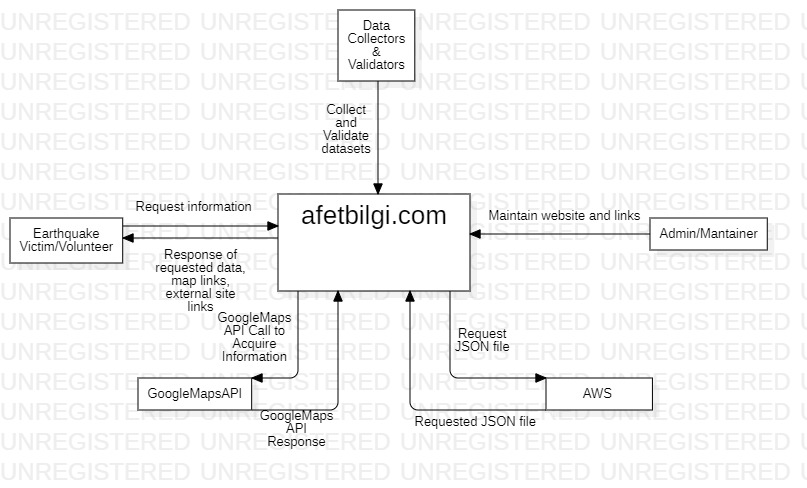
\includegraphics[width=\textwidth]{img/context-diagram.jpg}
  \caption{Context Diagram for \href{https://afetbilgi.com}{afetbilg.com}}
\end{figure}

\subsubsection{System Functions}

\subsubsection{Stakeholder Characteristics}

\subsubsection{Limitations}

\subsection{Definitions}


\section{References}


\section{Glossary}

\begin{table}[H]
  \centering
  \resizebox{\linewidth}{!}{%
    \begin{tabular}{|p{.3\linewidth}|p{.7\linewidth}|}
      \hline
      \textbf{Term} & \textbf{Definition} \\ \hline
      Python & Computer Programming language to create applications, features, etc. \\ \hline
      React & A JavaScript framework widely used to create websites \\ \hline
      JavaScript & Scripting programming language used to create applets for the internet \\ \hline
      CI/CD & Continuous Integration/Continuous Development \\ \hline
      HTTPS & An internet protocol known as Hyper Text Transfer Protocol Secured \\ \hline
      AWS & Amazon Web Services the provide web hosting servicing \\ \hline
      CloudFlare & A secure DNS hosting service \\ \hline
      Vercel & A web hosting service \\ \hline
      UI/UX & User Interface/User Experience, meant to refer to the frontend part of a web app that the target audience of the website interact with \\ \hline
      PDF & Known as Portable Document Format for easy sharing \\ \hline
      IP & Internet Protocol \\ \hline
      DNS & Domain Name Server \\ \hline
      AWS IAM & Amazon Web Services Identity and Access Management is a service that enables you to manage access to AWS resources securely by creating and managing users, groups, and roles with assigned permissions. \\ \hline
    \end{tabular}
  }
  \caption{Glossary of Terms}
\end{table}


\section{Architectural Views}

\subsection{Context View}

\subsubsection{Stakeholders' Uses of This View}

\subsubsection{Context Diagram}

% Checked in grammarly
\afetbilgi \cite{afetbilgi} is not part of a more extensive system. It is a standalone and open-source efforted website to verify critical information in the fight against the 6 February 2023 Pazarcik Earthquake and deliver it to disaster victims and those who want to help in an understandable, concise manner in multiple languages.

This information is presented in either the form of legible tables with third-party governmental and private links or an interactable method via a map view interface. If deemed necessary, admin and maintainers can make changes to display newly created or edited data and upload it to the system upon any complaints or suggestions they may get on their contact details.

\begin{figure}[H]
  \centering
  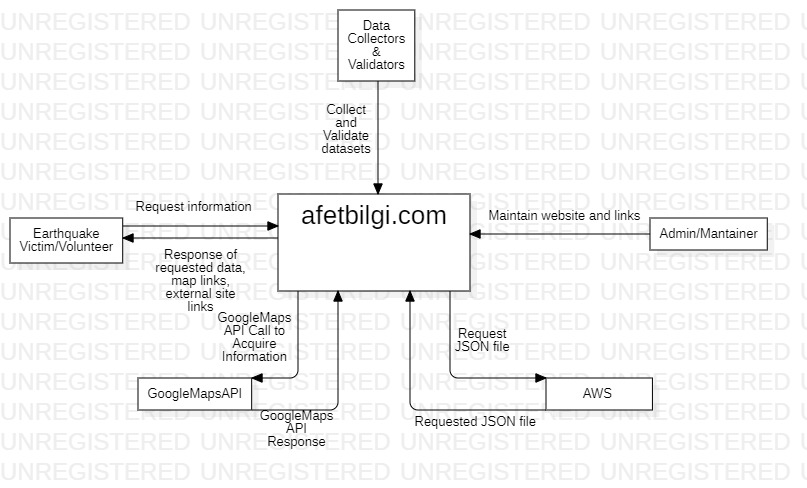
\includegraphics[width=\linewidth]{img/context-diagram.jpg}
  \caption{Context Diagram for \afetbilgi}
\end{figure}

The \afetbilgi\ consists of a combination of small physical and software parts. With the help of interfaces, these parts communicate among themselves and with the user.

\subsubsection{External Interfaces}

\begin{figure}[H]
  \centering
  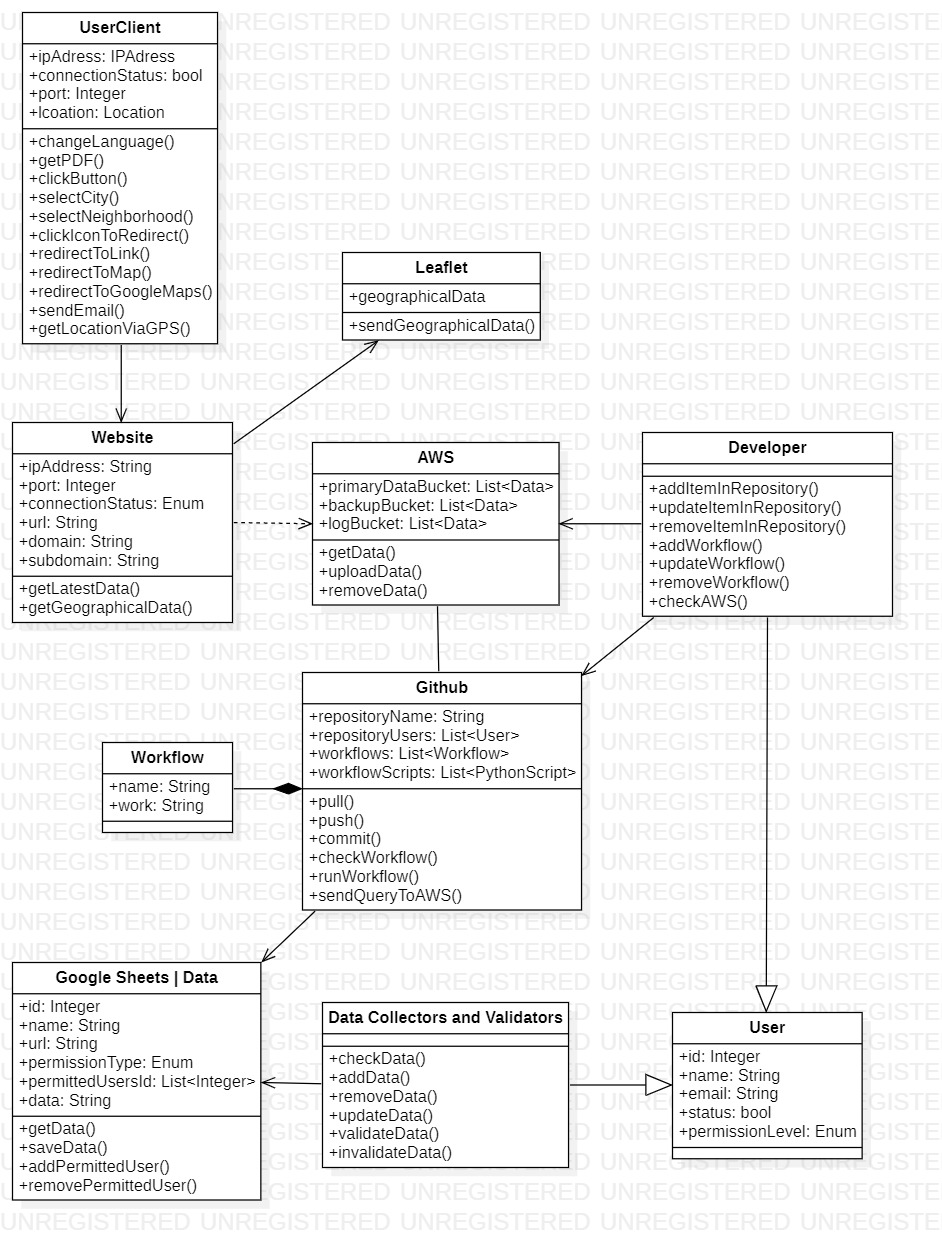
\includegraphics[width=\linewidth]{img/external-interfaces-diagram.jpg}
  \caption{External Interfaces}
\end{figure}

\subsubsection{Interaction Scenarios}

\begin{figure}[H]
  \centering
  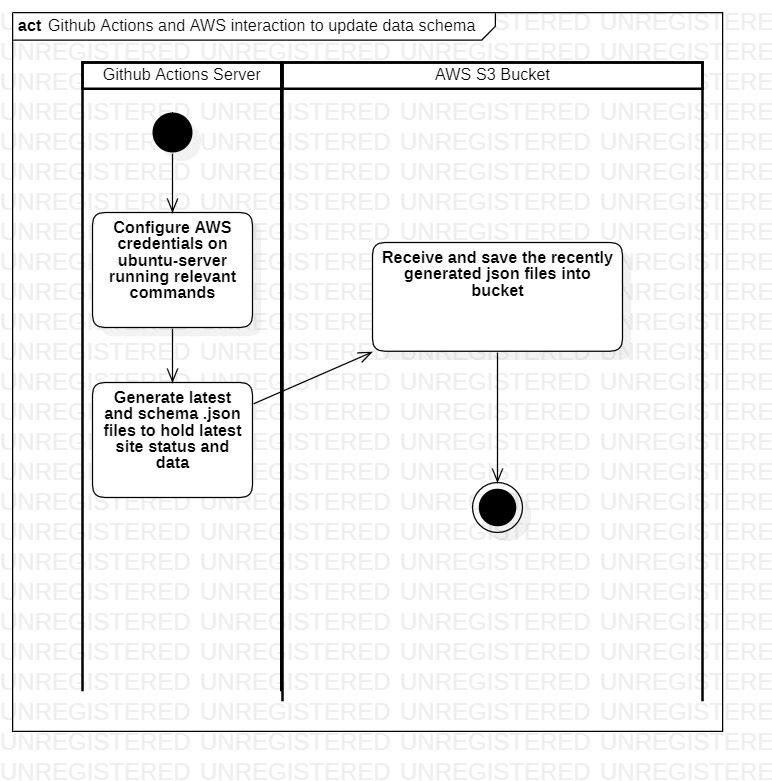
\includegraphics[width=\linewidth]{img/activity-diagram-1.jpg}
  \caption{Activity Diagram | GitHub Actions and AWS Interaction to Update Data Schema}
\end{figure}

\begin{figure}[H]
  \centering
  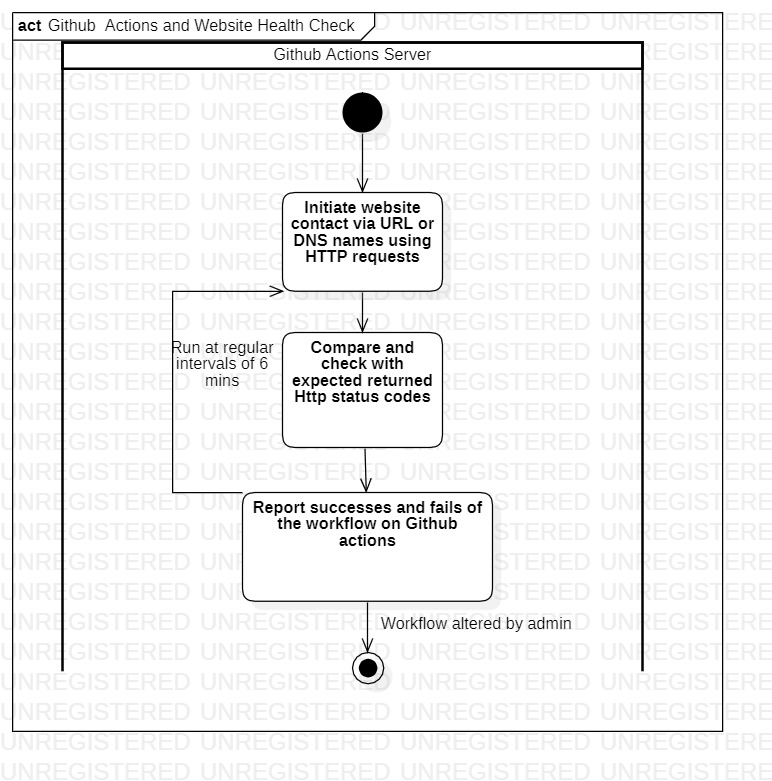
\includegraphics[width=\linewidth]{img/activity-diagram-2.jpg}
  \caption{Activity Diagram | GitHub Actions and Website Health Check}
\end{figure}

\subsection{Functional View}

\subsubsection{Stakeholders' Uses of This View}

\subsubsection{Component Diagram}

\begin{figure}[H]
  \centering
  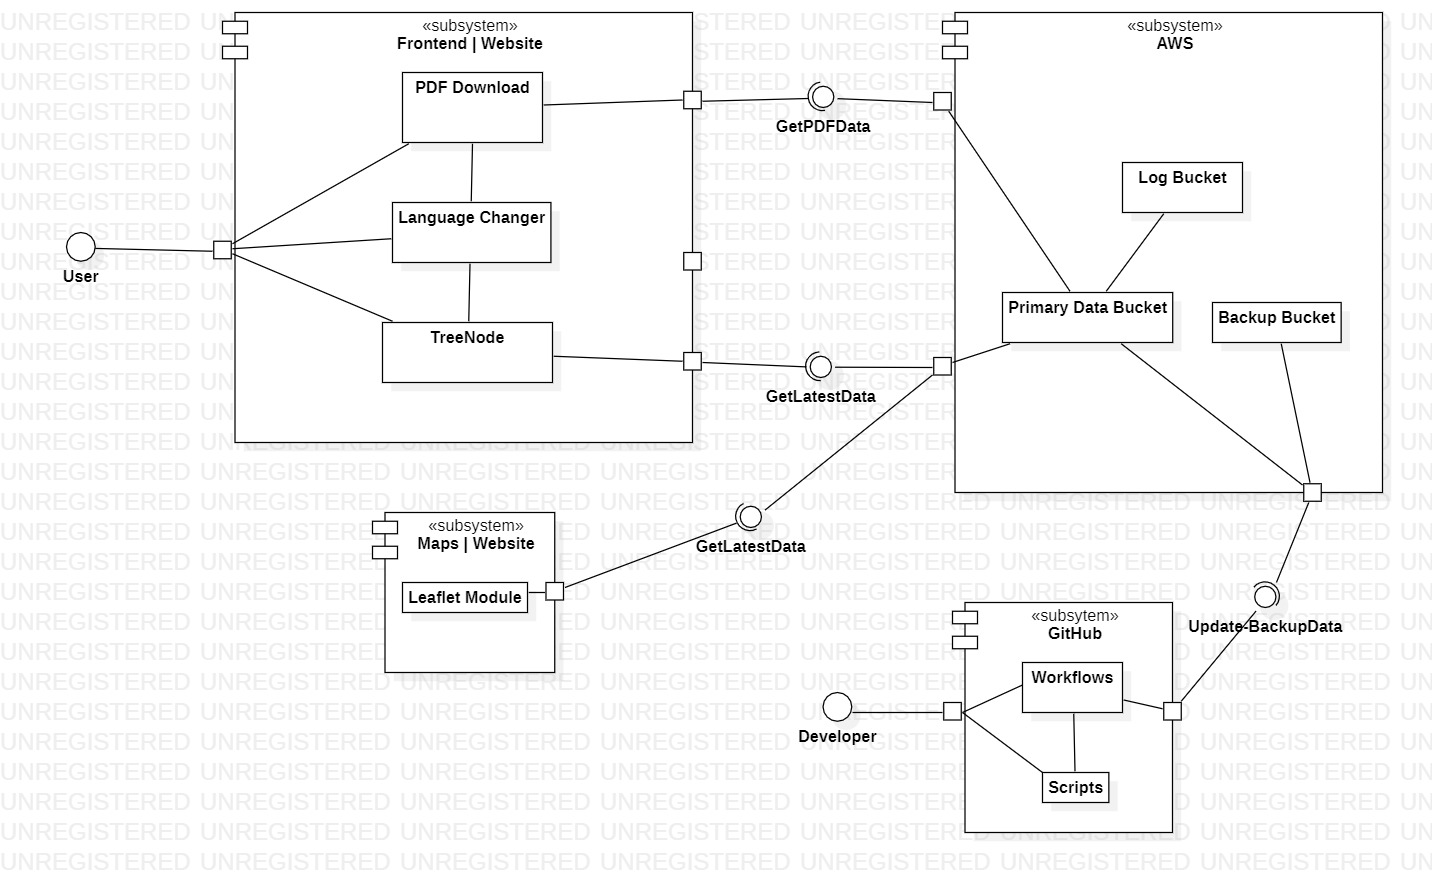
\includegraphics[width=\linewidth]{img/component-diagram.jpg}
  \caption{Component Diagram}
\end{figure}

\subsubsection{Internal Interfaces}

\begin{figure}[H]
  \centering
  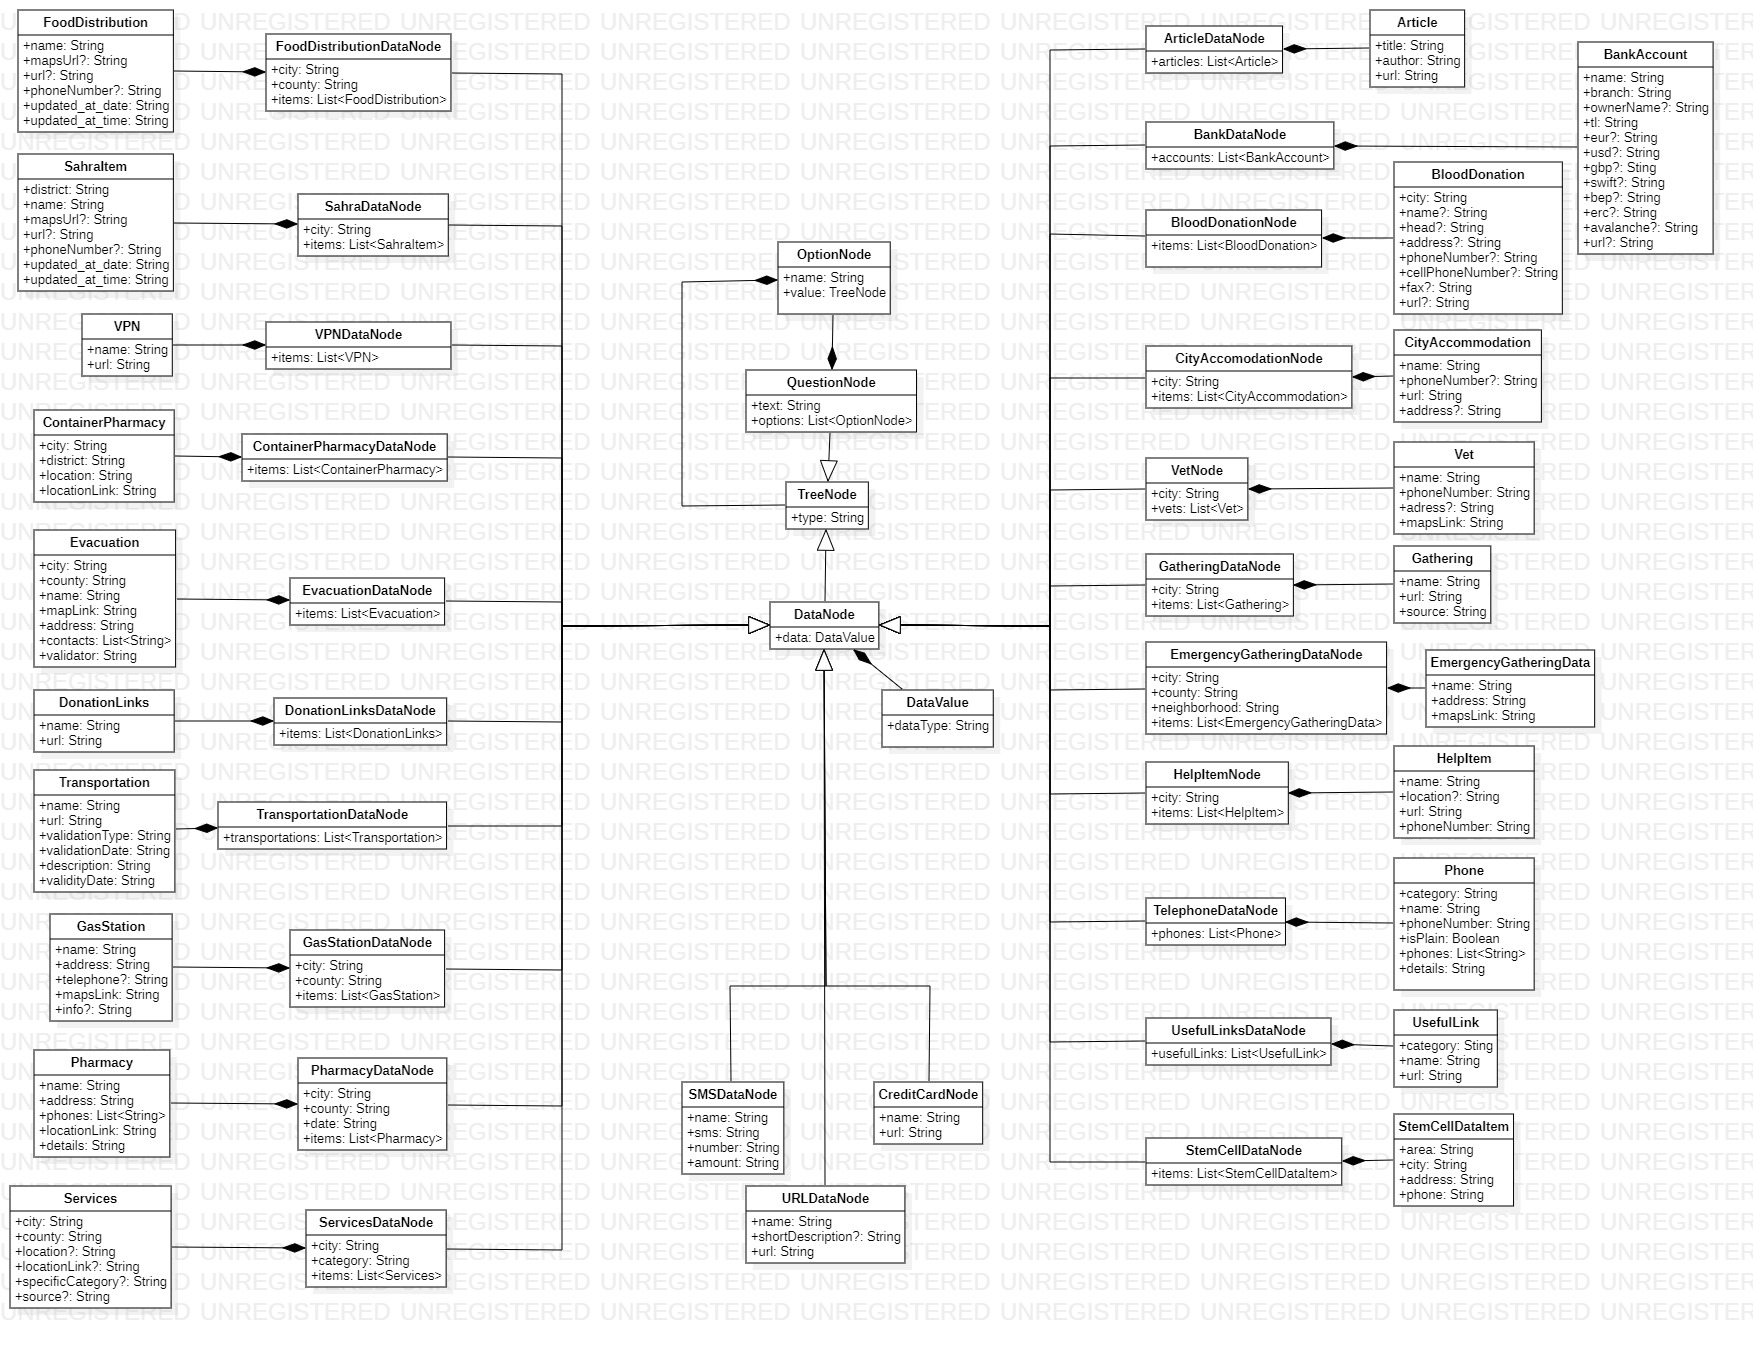
\includegraphics[width=\linewidth]{img/internal-interfaces-diagram.jpg}
  \caption{Internal Interfaces}
\end{figure}

\subsubsection{Interaction Patterns}

\begin{figure}[H]
  \centering
  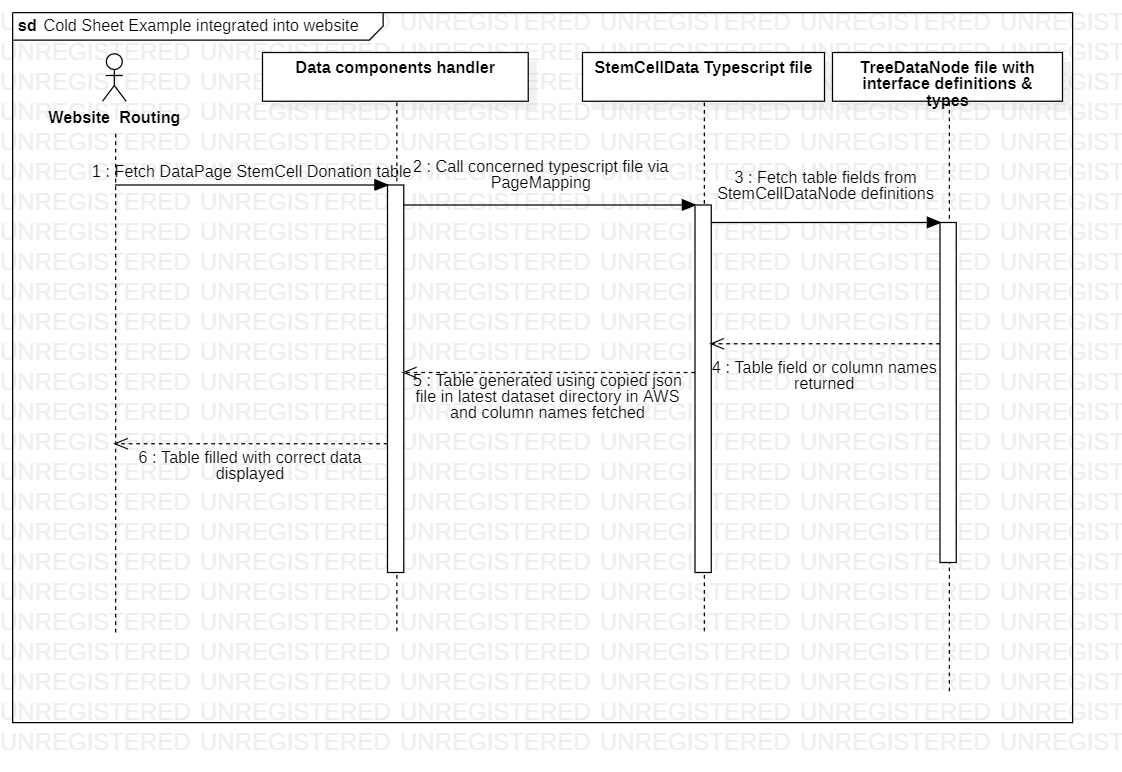
\includegraphics[width=\linewidth]{img/sequence-diagram-1.jpg}
  \caption{Sequence Diagram | Cold Sheet Example Integrated Into Website}
\end{figure}

\begin{figure}[H]
  \centering
  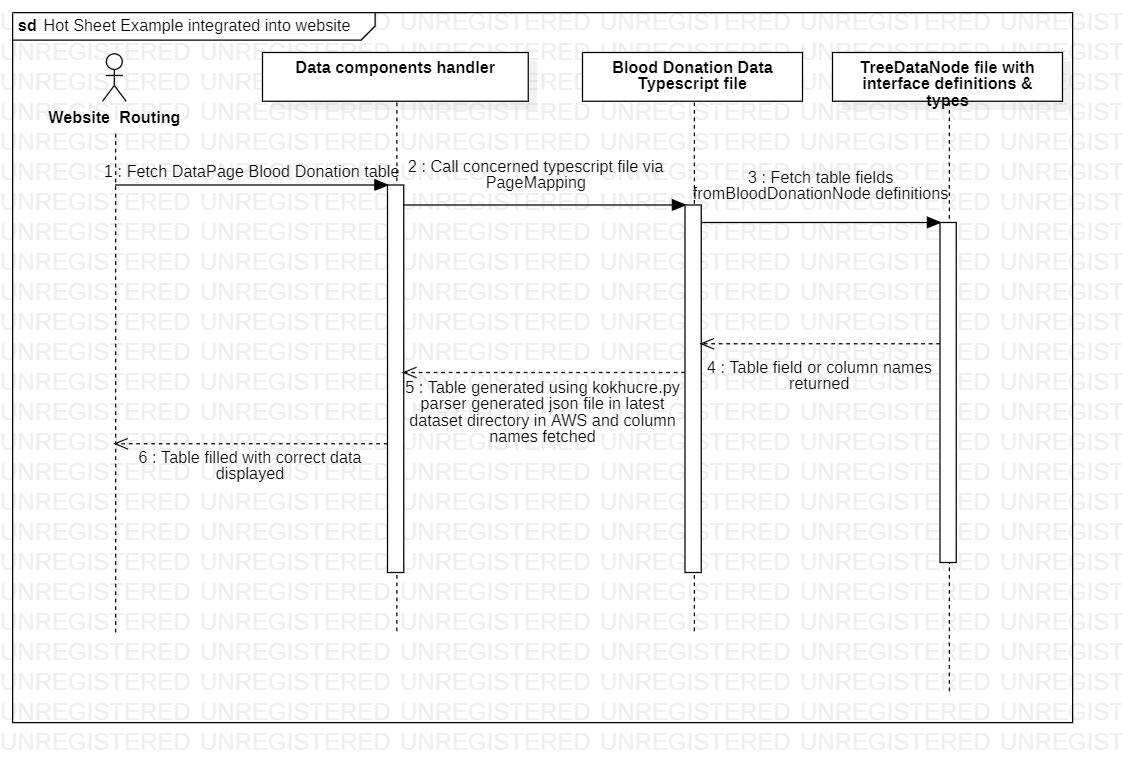
\includegraphics[width=\linewidth]{img/sequence-diagram-2.jpg}
  \caption{Sequence Diagram | Hot Sheet Example Integrated Into Website}
\end{figure}

\begin{figure}[H]
  \centering
  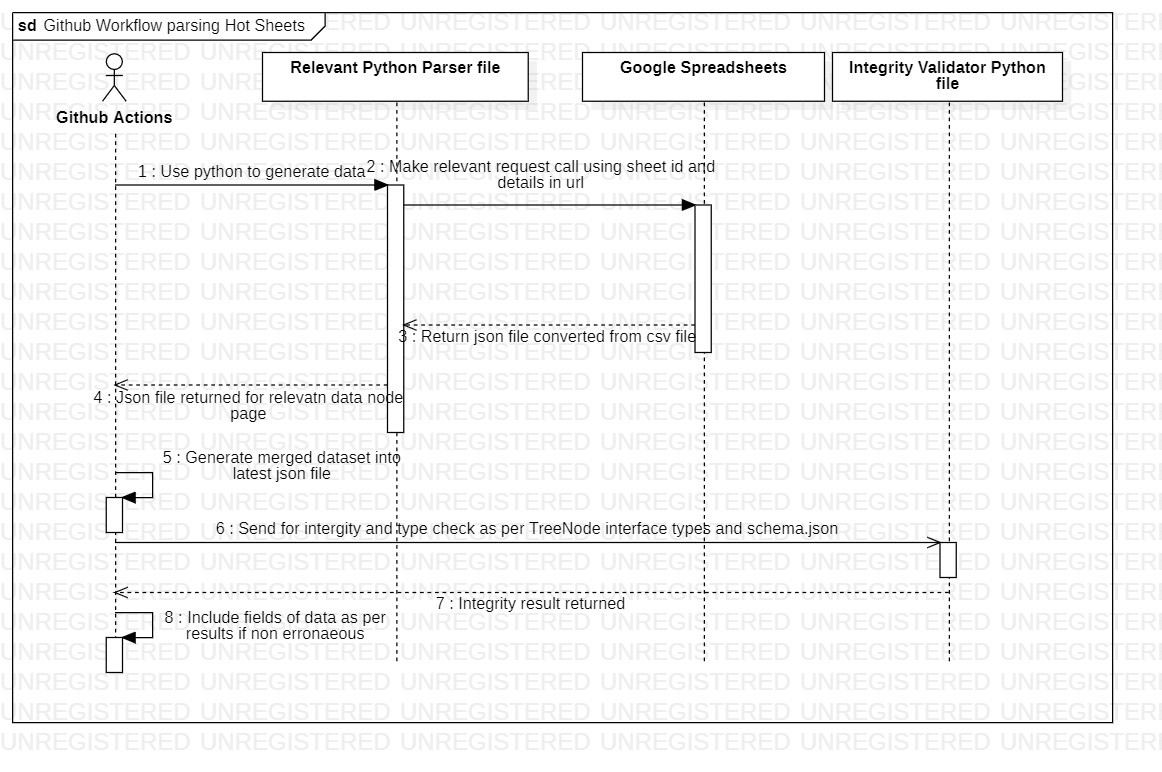
\includegraphics[width=\linewidth]{img/sequence-diagram-3.jpg}
  \caption{Sequence Diagram | GitHub Workflow Parsing Hot Sheets}
\end{figure}

\subsection{Information View}

\subsubsection{Stakeholders' Uses of This View}

\subsubsection{Database Class Diagram}

\begin{figure}[H]
  \centering
  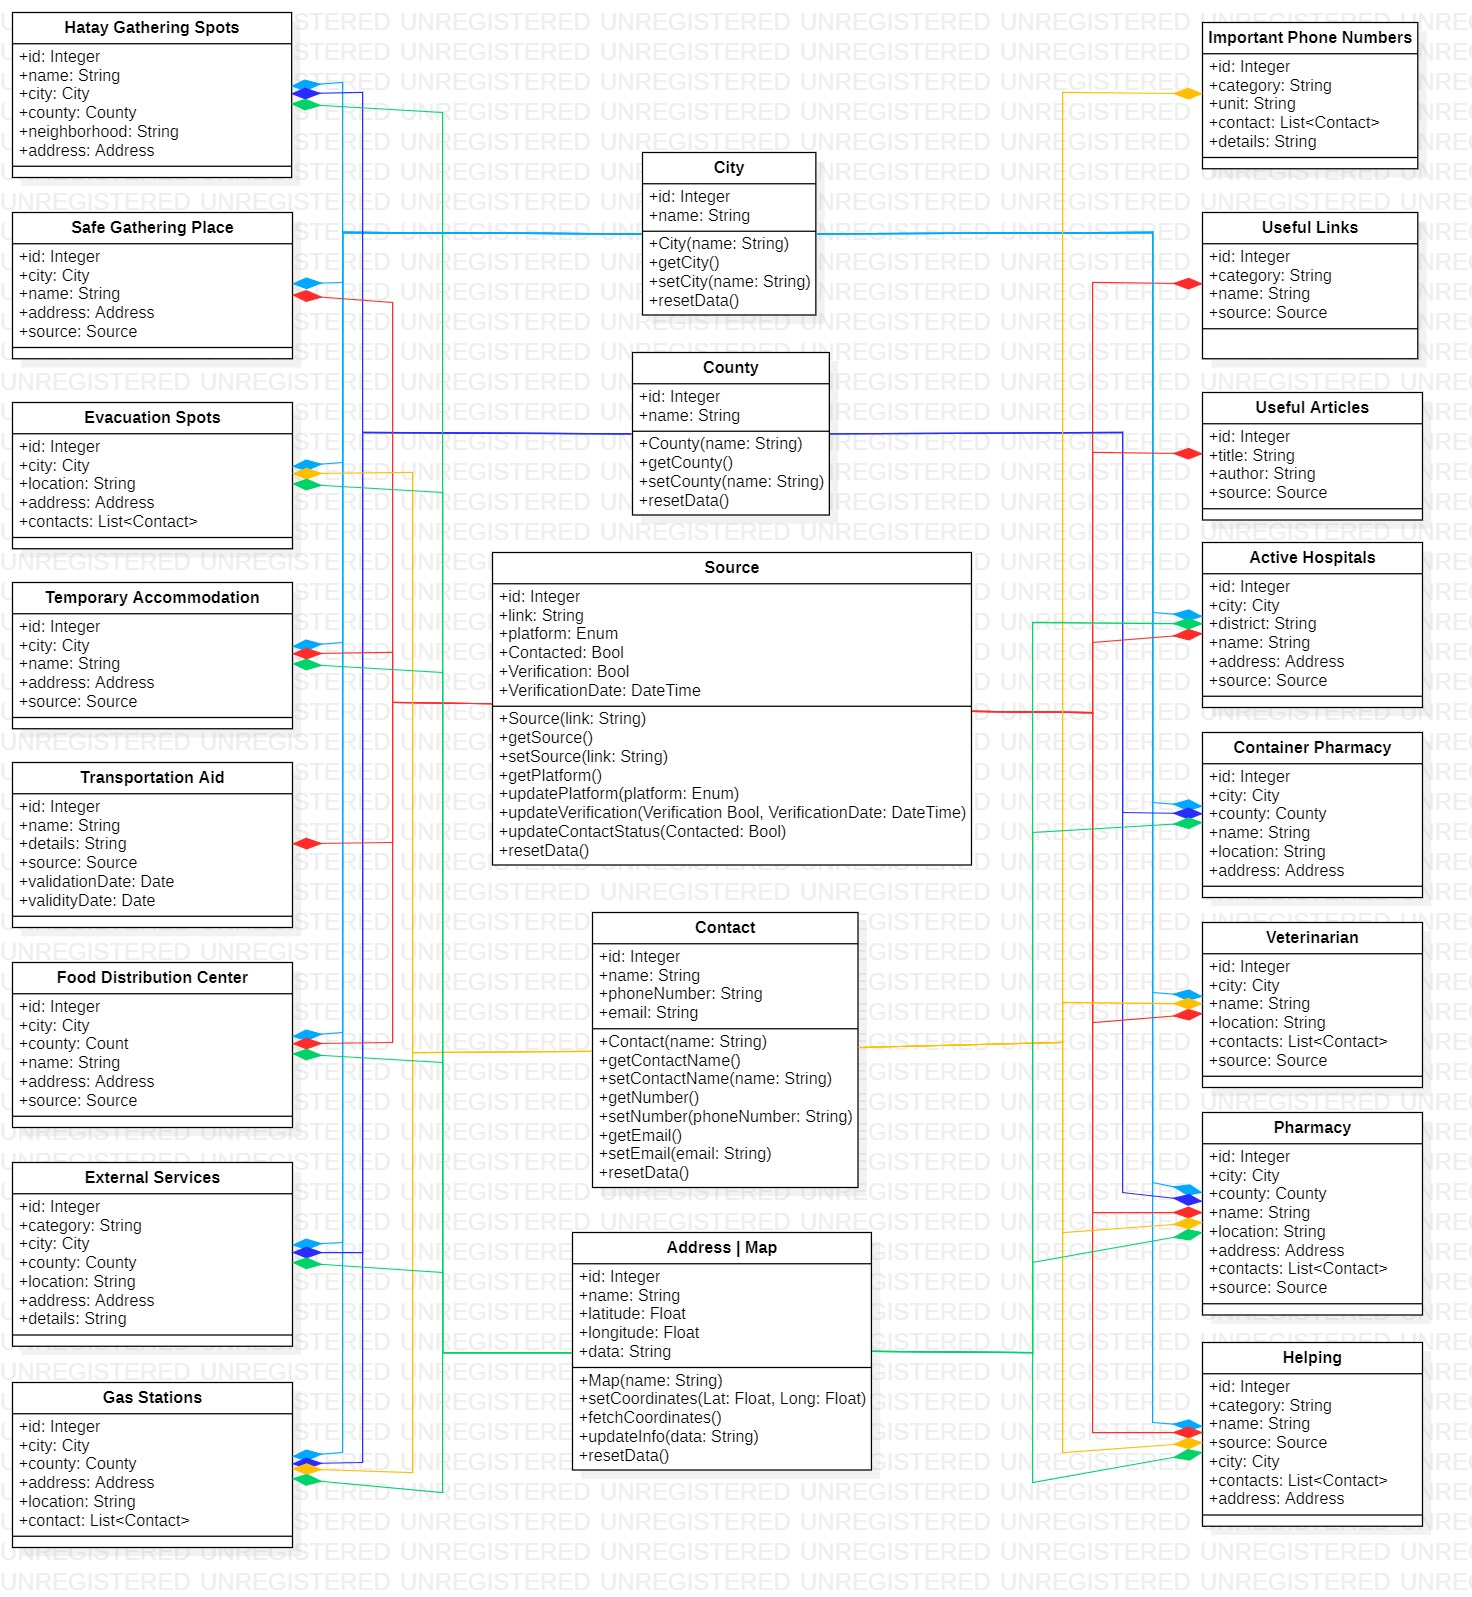
\includegraphics[width=\linewidth]{img/database-class-diagram.jpg}
  \caption{Database Class Diagram}
\end{figure}

\subsubsection{Operations on Data}

\subsection{Deployment View}

\subsubsection{Stakeholders' Uses of This View}

\subsubsection{Deployment Diagram}

\begin{figure}[H]
  \centering
  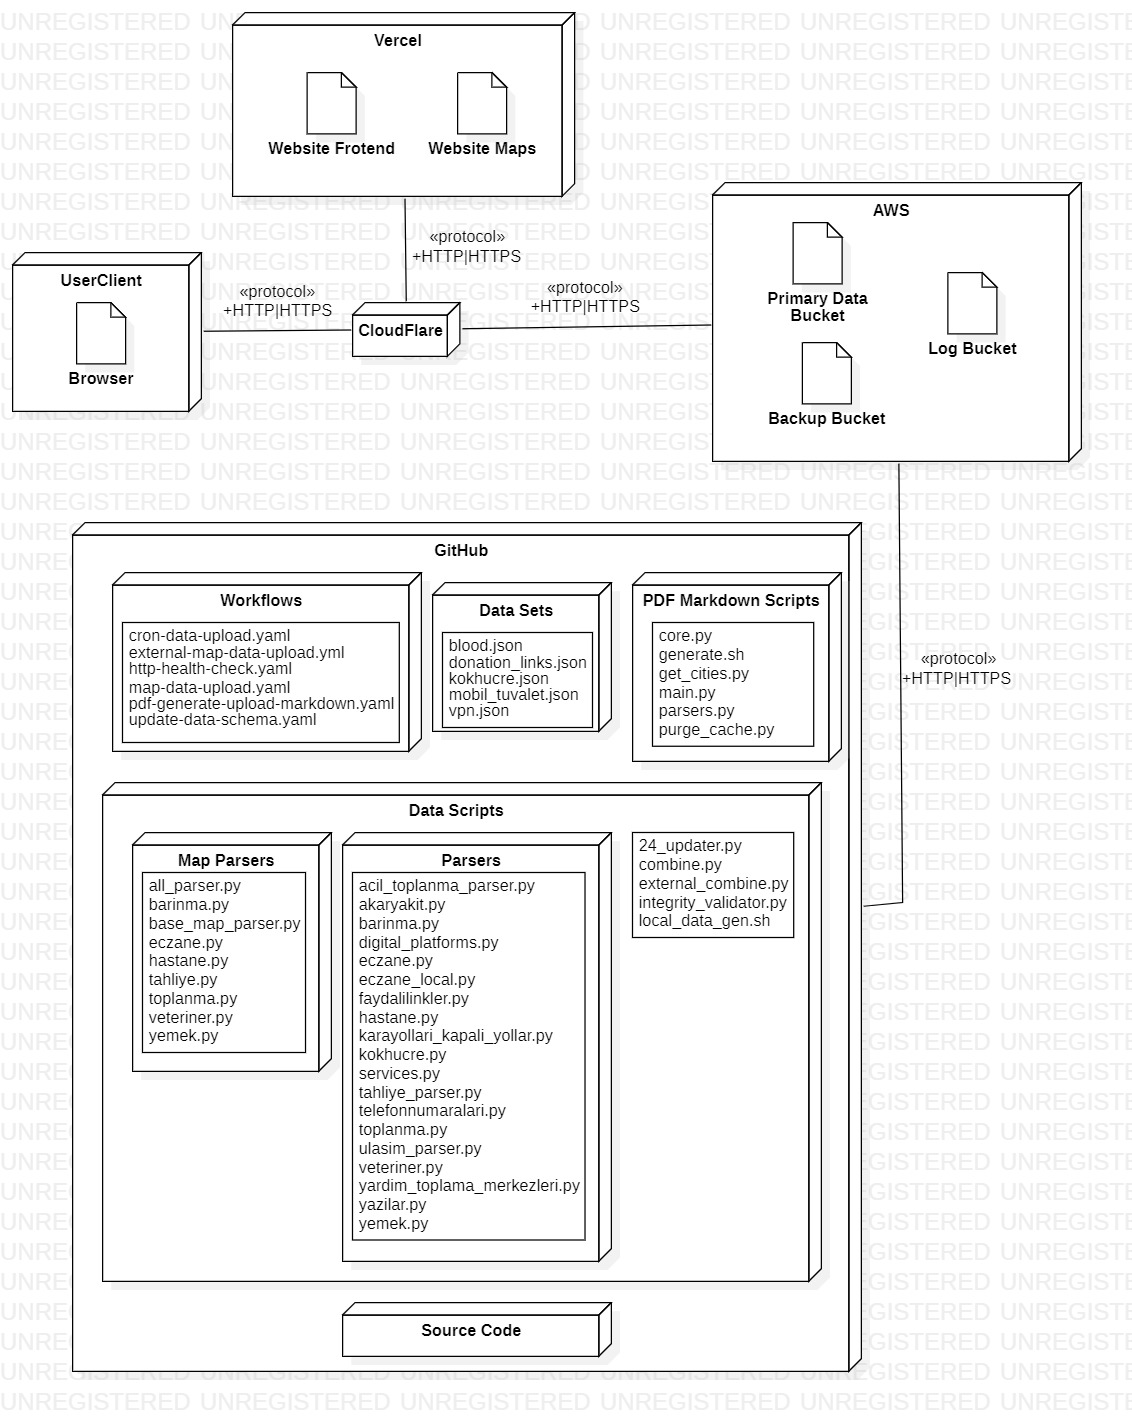
\includegraphics[width=\linewidth]{img/deployment-diagram.jpg}
  \caption{Deployment Diagram}
\end{figure}

\subsection{Design Rationale}


\newpage

\section{Architectural Views for Suggestions to Improve the Existing System}

\subsection{Context View}

\subsubsection{Stakeholders' Uses of This View}

In this view, system context is provided, with the actors and other systems related to it in a general manner. Website maintainers and Data collections of \afetbilgi\ will be the ones that primarily use this view to better understand how the different actors interact in the working of this website and the relationship that the system has with other external entities like the AWS components, Maps API component, and so on. In addition, Authentication has been added and can use Google API as a reliable 3rd party user registration handling as well along with an embedded Mail subscription handling module to inform users of potential alerts given the ongoing emergency situation about the earthquake.  Similar interfaces are further explained in our added components in the external diagram. 

\vspace*{\fill}
\newpage

\subsubsection{Context Diagram}

\afetbilgi\ is not part of a more extensive system. It is a standalone and open-source efforted website to verify critical information in the fight against the 6 February 2023 Pazarcik Earthquake and deliver it to disaster victims and those who want to help in an understandable, concise manner in multiple languages.

This information is presented in either the form of legible tables with third-party governmental and private links or an interactable method via a map view interface. If deemed necessary, admin and maintainers can make changes to display newly created or edited data and upload it to the system upon any complaints or suggestions they may get on their contact details.

\begin{figure}[H]
  \centering
  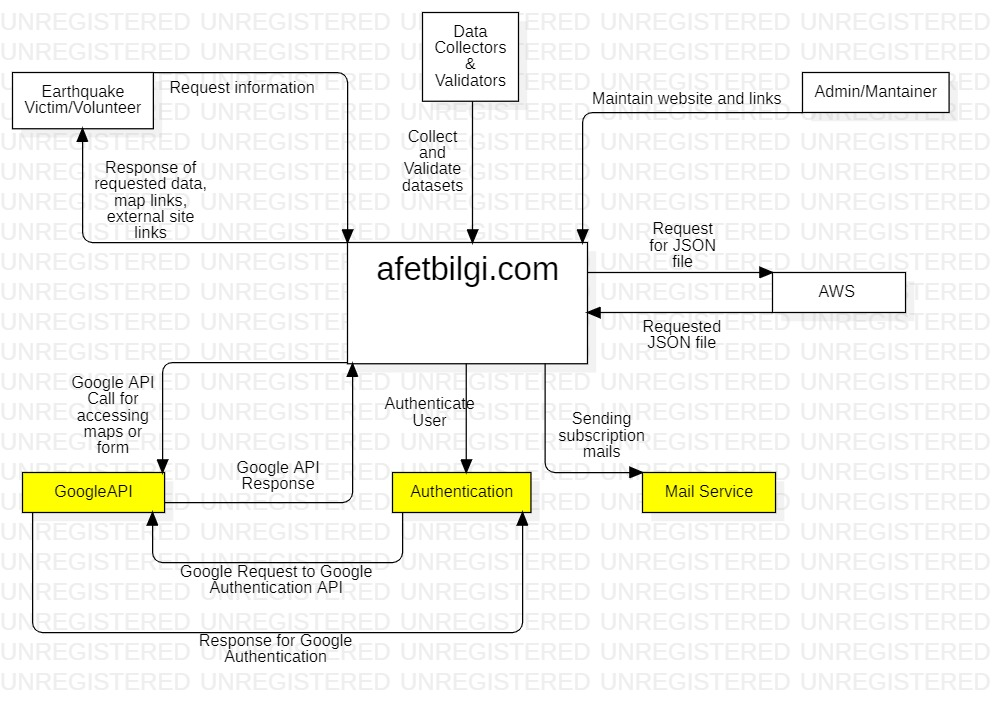
\includegraphics[width=\linewidth]{img/context-diagram-s5.jpg}
  \caption{Suggested Context Diagram}
\end{figure}

The \afetbilgi\ consists of a combination of small physical and software parts. With the help of interfaces, these parts communicate among themselves and with the user.

\subsubsection{External Interfaces}

\begin{figure}[H]
  \centering
  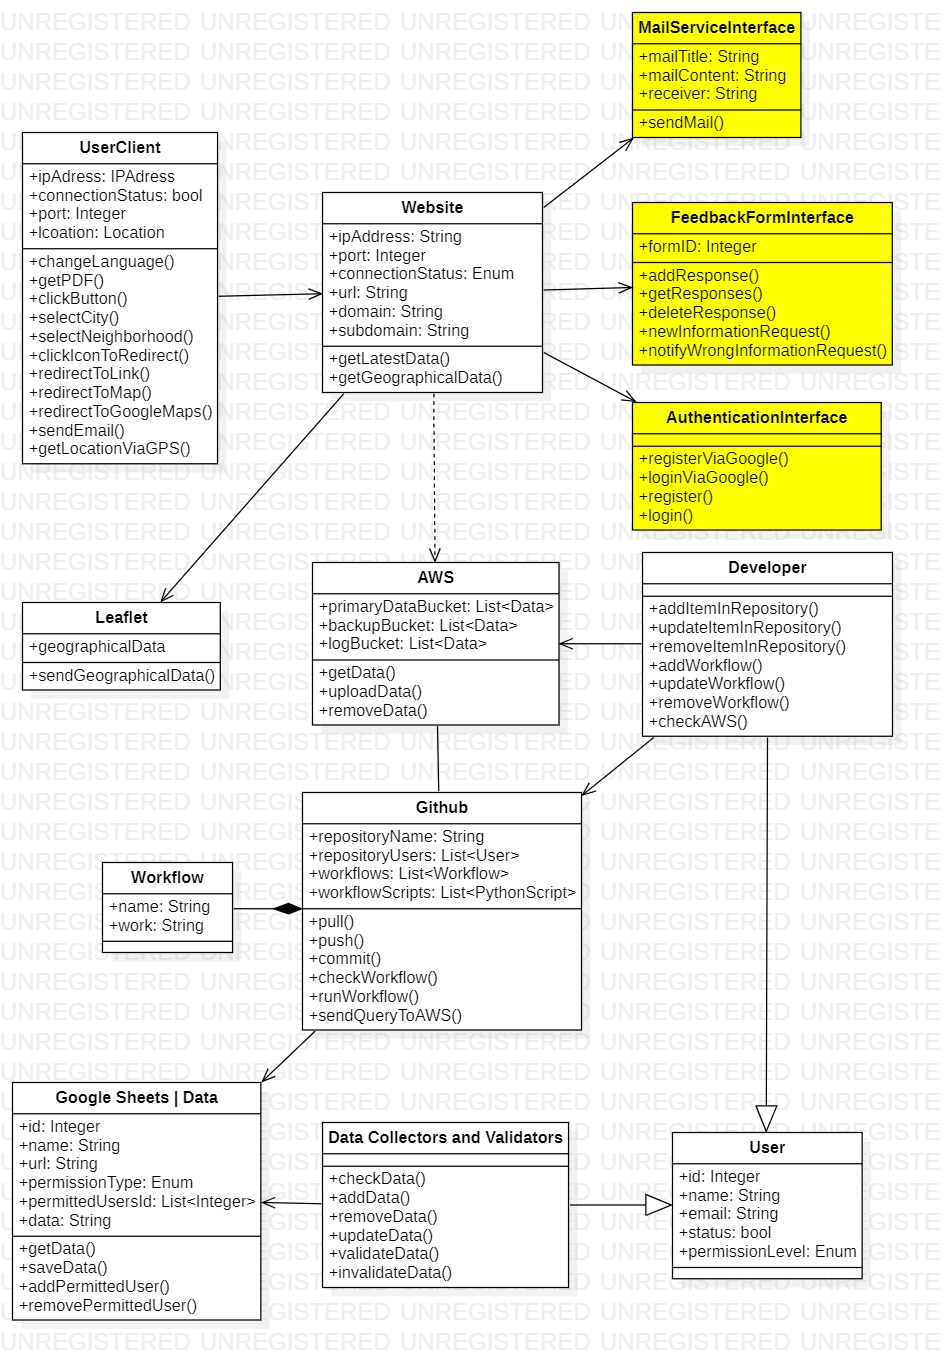
\includegraphics[width=\linewidth]{img/external-interfaces-diagram-s5.jpg}
  \caption{Suggested External Interfaces Diagram}
\end{figure}

As it can be observed from Figure \addnumbertofigure{0}, \afetbilgi\ has multiple external interfaces. We have added MailServiceInterface, FeedbackFormInterface and AuthenticationInterface. The operations given in the diagram can be summarized as follows:
\begin{itemize}
  \item MailServiceInterface provides the option of sending mail about the updated information to the subscribed users.
  \item FeedbackFormInterface provides the option of sending feedback related to website and the data. Users from the earthquake region can request for adding new information and notifying the wrong and expired infromation.
  \item AuthenticationInterface provides the option of logging in. The authentication system is used to provide opportunity to authorized institutions and organizations to update the information from the website directly.
\end{itemize}

\subsubsection{Interaction Scenarios}

\begin{figure}[H]
  \centering
  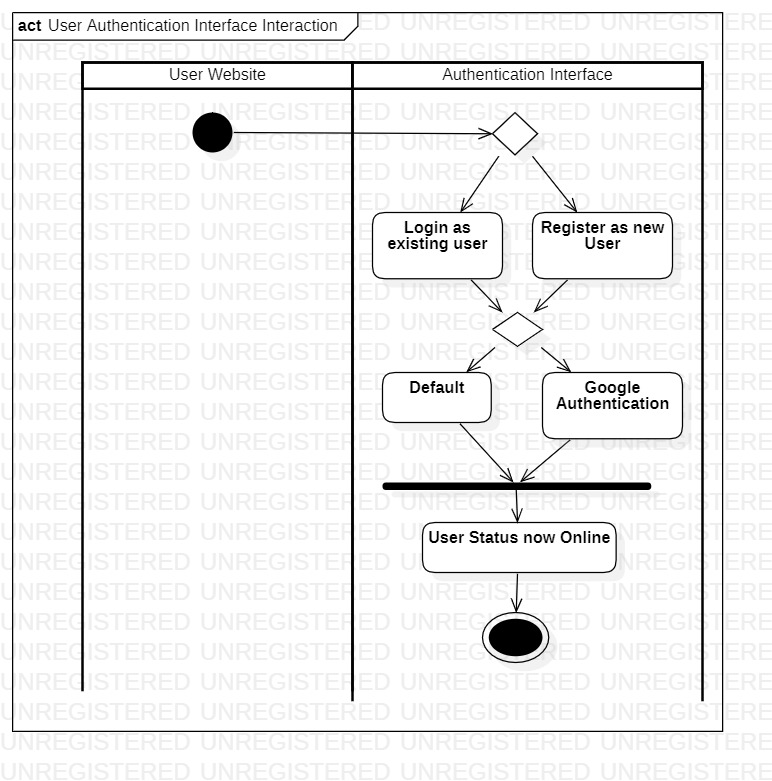
\includegraphics[width=\linewidth]{img/activity-diagram-1-s5.jpg}
  \caption{Activity Diagram | User Authentication Interface Interaction}
\end{figure}

\subsection{Functional View}

\subsubsection{Stakeholders' Uses of This View}

This view depicts the different components of the system and their interaction, including the internal interfaces. This is extremely important for the stakeholders as it gives information about the system’s functionalities and the integral properties, it also gives way for other viewpoints and diagrams. As such victims and volunteers wont find this useful but website maintainers along with Data collectors would deeply appreciate this view to understand internal components and perhaps come up with ways to improve it. Additional components such as Google authentication would be handled by external API request to handle user registration as well another internal component to handle mail subscription to registered users. Similar new internal interfaces handle these arrears and interact with these additional external components.

\subsubsection{Component Diagram}

\begin{figure}[H]
  \centering
  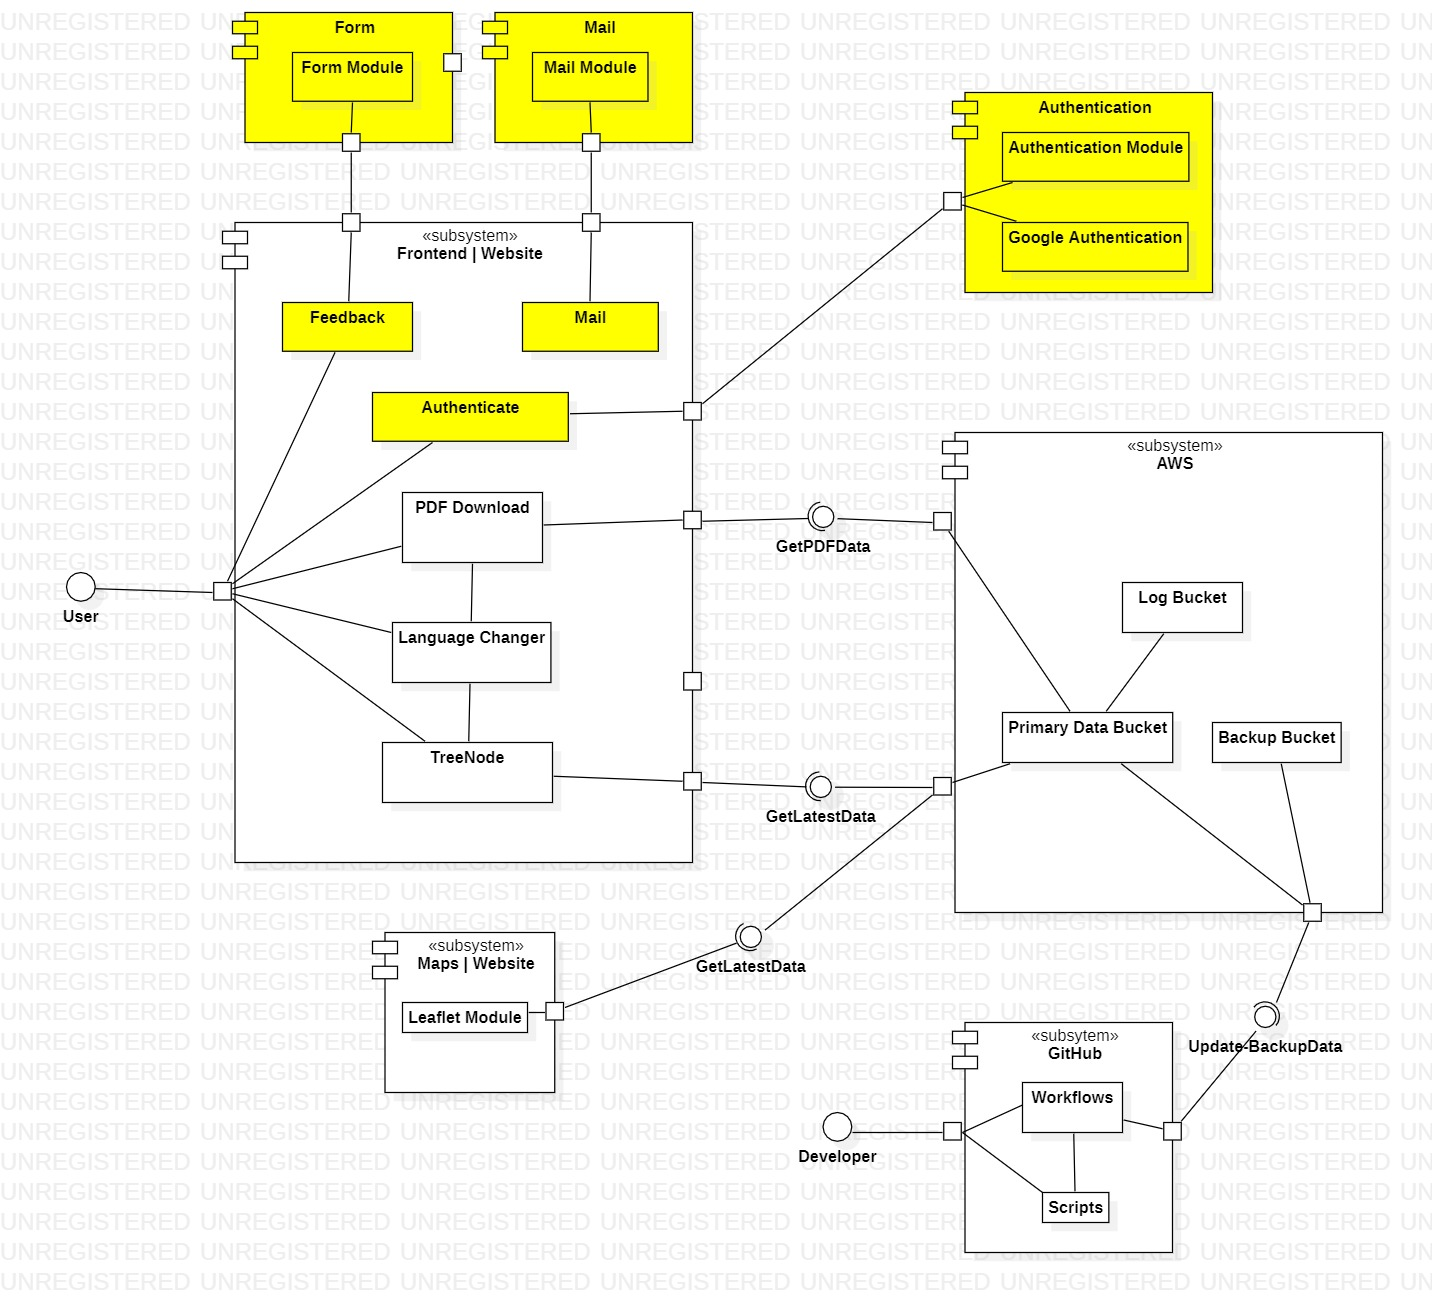
\includegraphics[width=\linewidth]{img/component-diagram-s5.jpg}
  \caption{Suggested Component Diagram}
\end{figure}

We have updated component diagram by adding the components for form, mail and authentication components:
\begin{itemize}
  \item Form provides user to send feedback about website and data so that the website and data can be updated according to the feedback by the normal users and victims.
  \item Mail component sends mail about the updated information to the subscribed users.
  \item Authentication component provide authorized users to register and login to the website by using Google Authentication system or built-in Authentication Module.
\end{itemize}

\subsubsection{Internal Interfaces}

\begin{figure}[H]
  \centering
  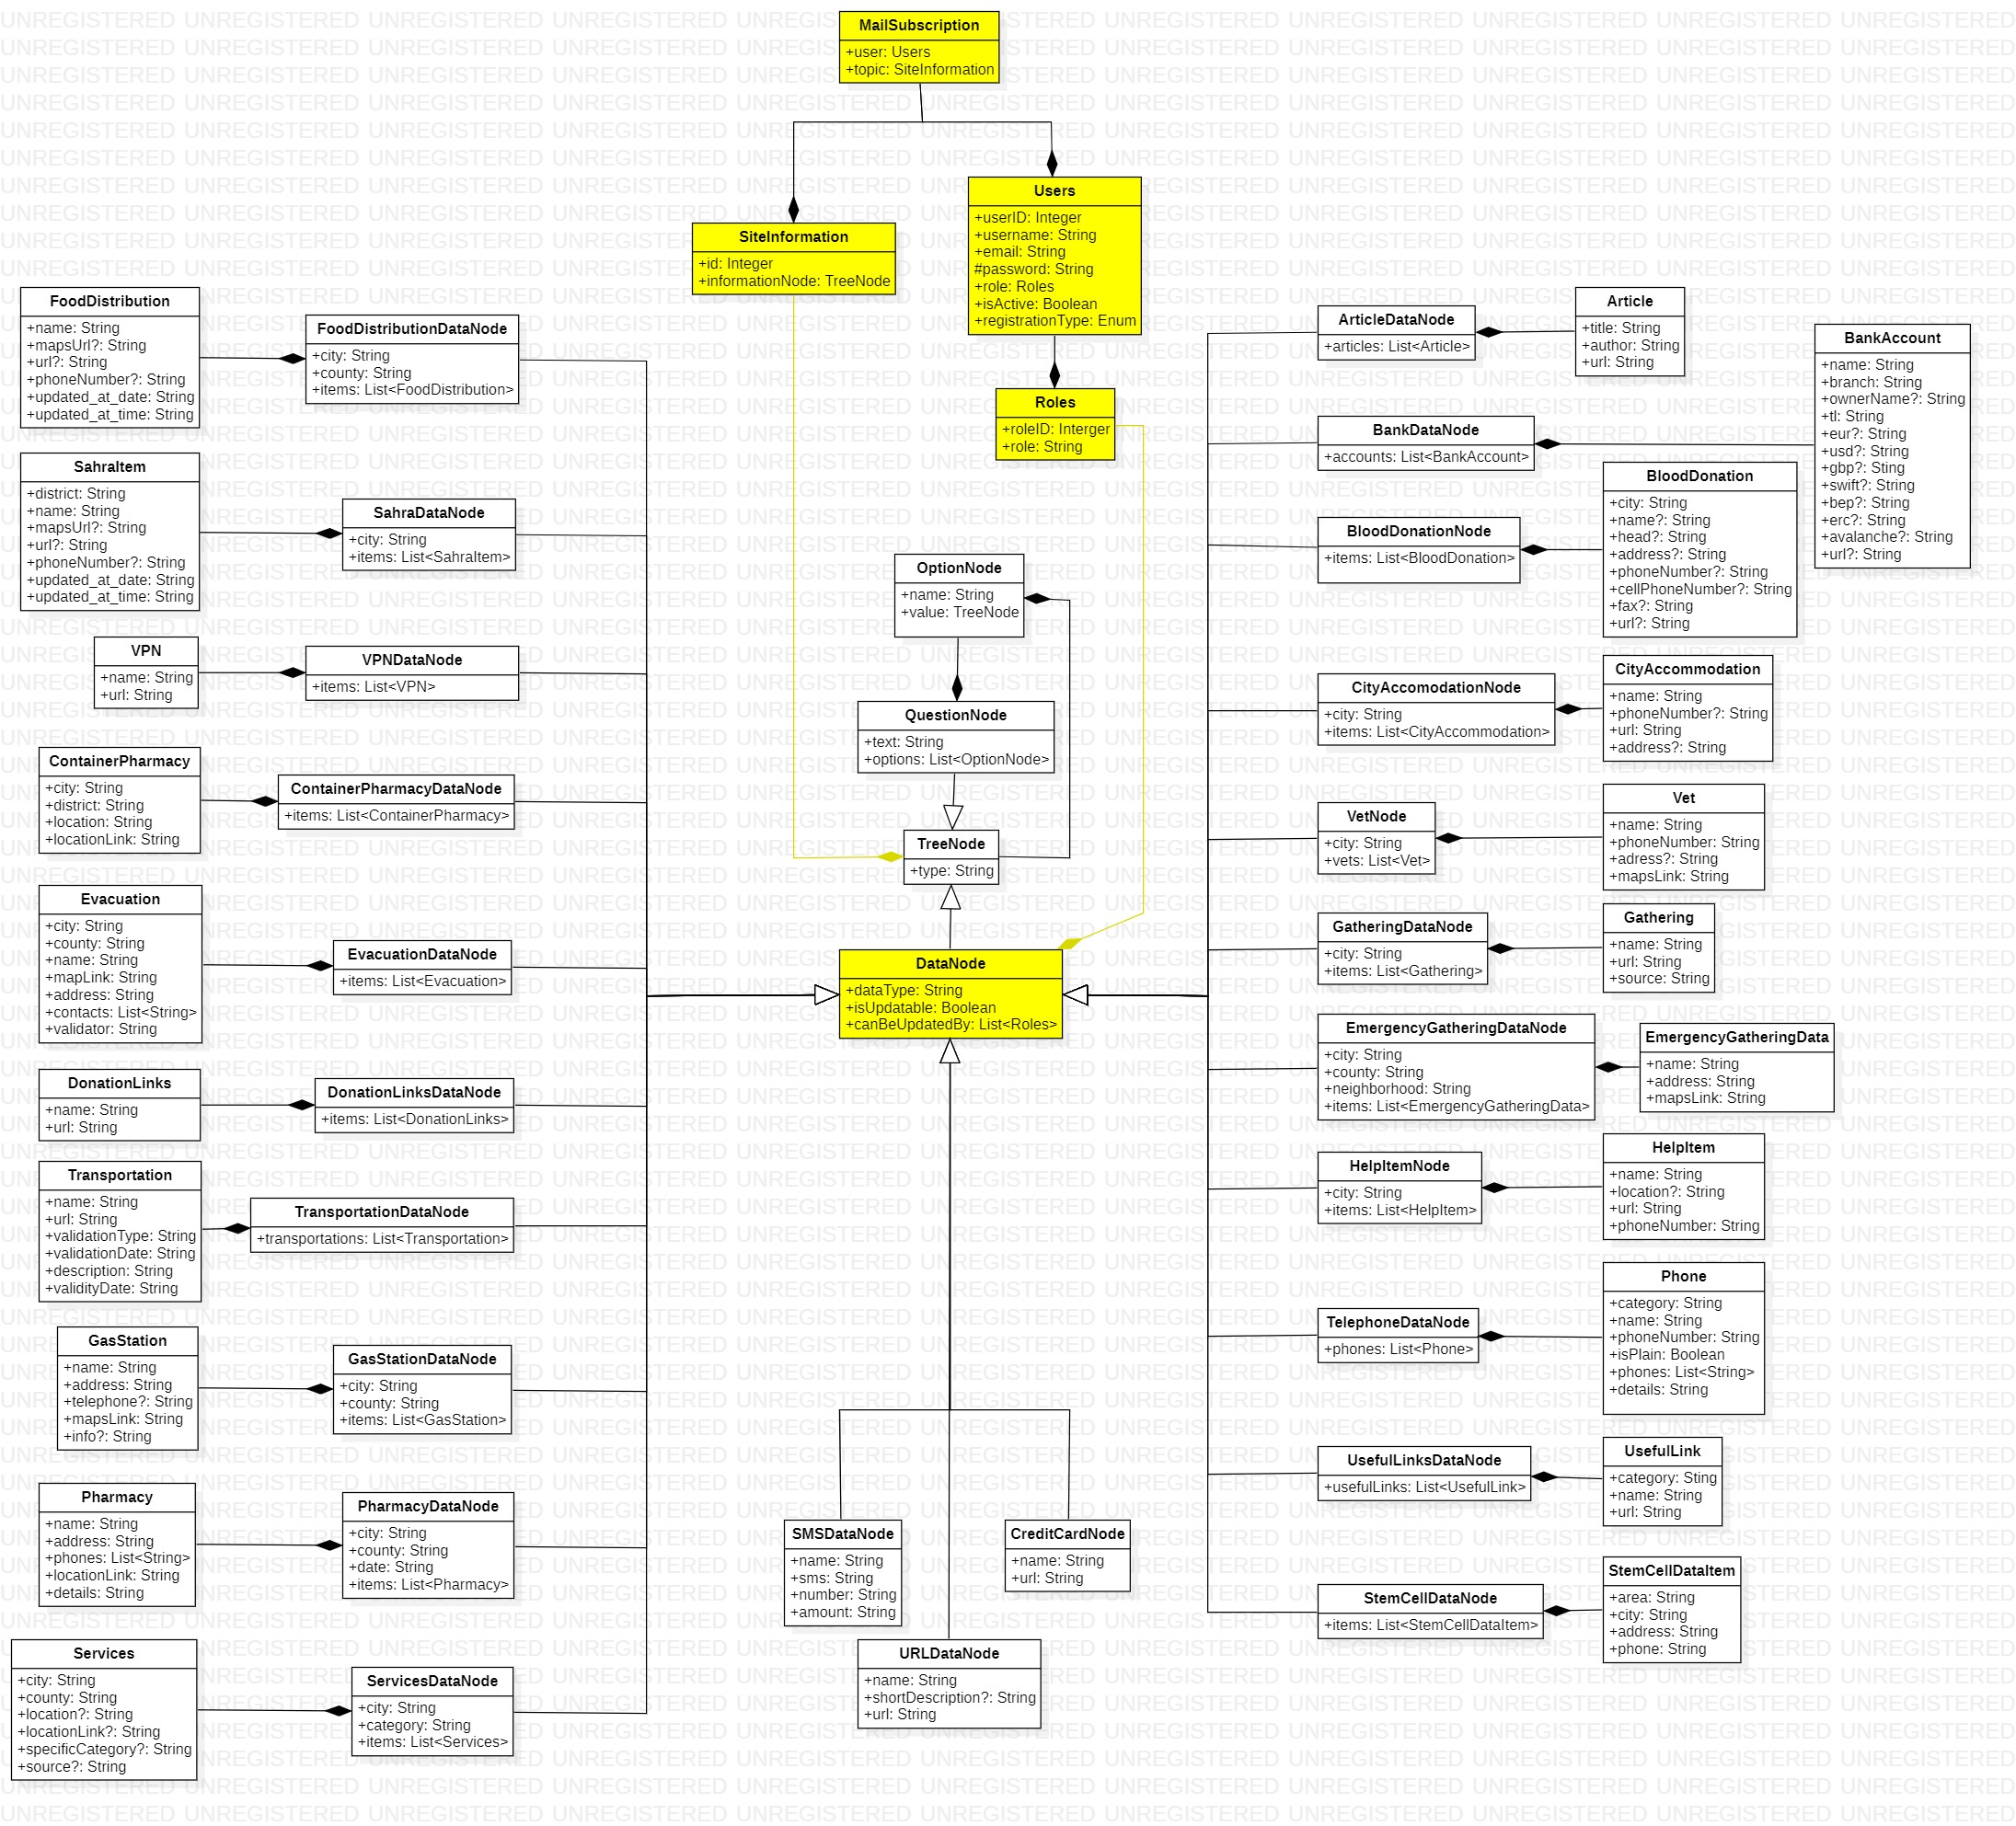
\includegraphics[width=\linewidth]{img/internal-interfaces-diagram-s5.jpg}
  \caption{Suggested Internal Interfaces}
\end{figure}


Since, there is no internal dynamism between interfaces initially, we embraced the same approches. Therefore, the internal interfaces are just the data interfaces to provide structured information for frontend code so that frontend code can parse the information correctly and fastly.

The main data is stored in the database and retrieved from database, so the frontend code parses the data.

\subsubsection{Interaction Patterns}

\begin{figure}[H]
  \centering
  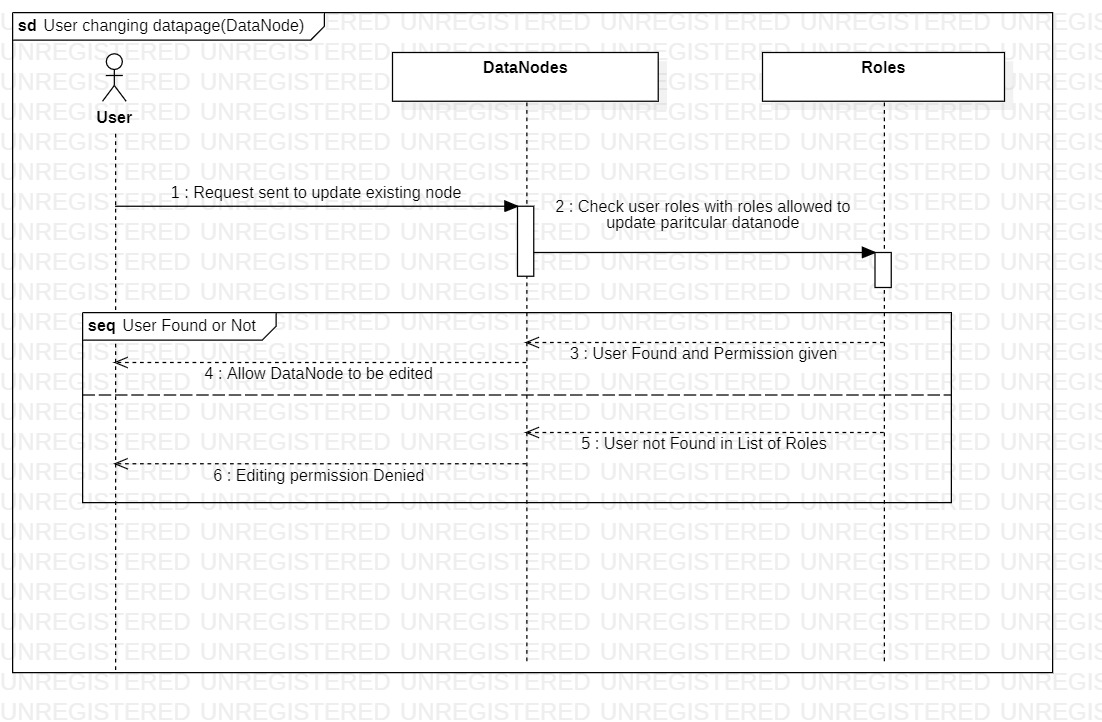
\includegraphics[width=\linewidth]{img/sequence-diagram-1-s5.jpg}
  \caption{Sequence Diagram | User Changing Datapage}
\end{figure}

\vspace*{\fill}
\newpage

\subsection{Information View}

\subsubsection{Stakeholders' Uses of This View}

This view concerns the variables and the data used and stored in this system during use as per Rozanski’s explanations. While this open-source, static and nondynamic website doesn’t employ a database infrastructure backend like mySQL, stakeholders such as website maintainers along with data maintainers/validators would again appreciate to know which data pages and nodes are being exchanged and whether any unreliable information is being or has been uploaded to the website assets and datasheets. In additional an essential user database class has been added with additional mail subscription classes to formalize and secure the website even further. As per allotted roles the user would have the autheorization to make changes onto the website.

\subsubsection{Database Class Diagram}

\begin{figure}[H]
  \centering
  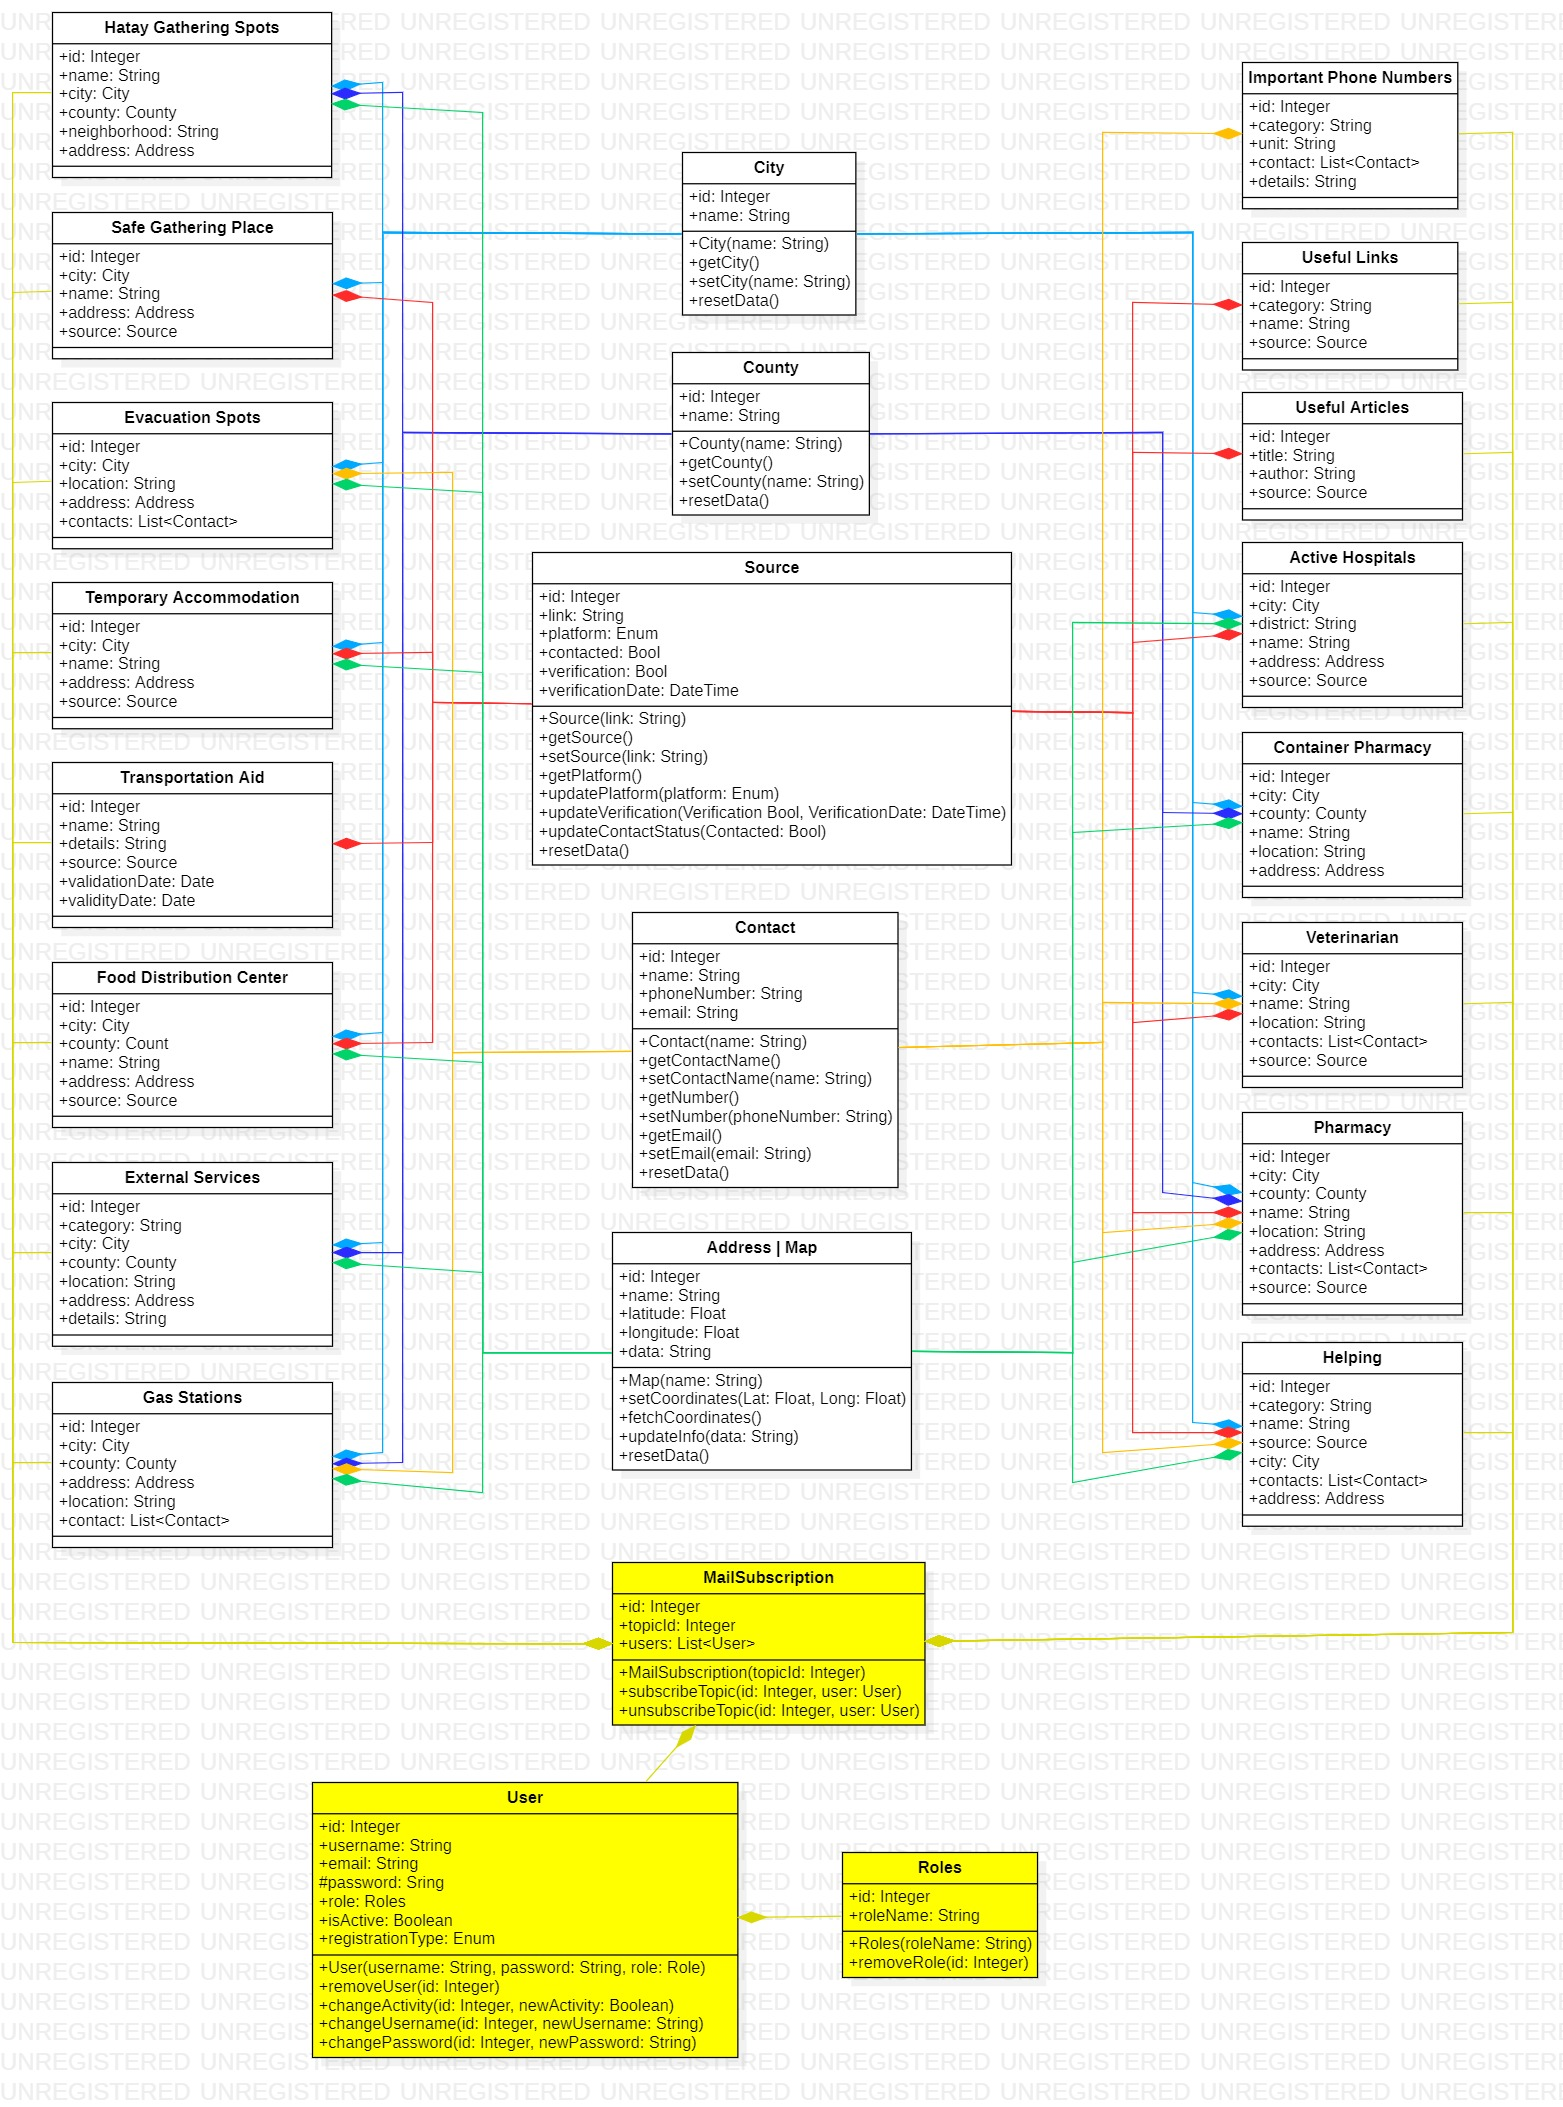
\includegraphics[width=\linewidth]{img/database-class-diagram-s5.jpg}
  \caption{Suggested Database Class Diagram}
\end{figure}

\subsubsection{Operations on Data}

\begin{longtable}{|p{.3\linewidth}|p{.7\linewidth}|}
    \hline
    New Operations & CRUD Operations \\ \hline
    % Burak's Part
    MailSubscription :: & Create: Create new MailSubscription item with given topicId \\
    MailSubscription()  & Read: \\
                        & Update: \\
                        & Delete: \\ \hline
    MailSubscription :: & Create: \\
    subscribeTopic()    & Read: \\
                        & Update: Add user to the users list of the subcription item \\
                        & Delete: \\ \hline
    MailSubscription :: & Create: \\
    unsubscribeTopic()  & Read: \\
                        & Update: Remove user from the users list of the subcription item \\
                        & Delete: \\ \hline

    User :: User() & Create: Create new user with given arguments \\
                 & Read: \\
                 & Update: \\
                 & Delete \\ \hline
    User :: removeUser() & Create: \\
                       & Read: \\
                       & Update: \\
                       & Delete: Delete user with given id \\ \hline
    User :: changeActivity() & Create: \\
                           & Read: \\
                           & Update: Update the activity status of the user \\
                           & Delete: \\ \hline
    User :: changeUsername() & Create: \\
                           & Read: \\
                           & Update: Update the username of the user \\
                           & Delete: \\ \hline
    User :: changePassword() & Create: \\
                           & Read: \\
                           & Update: Update the password of the user \\
                           & Delete: \\ \hline

    Roles :: Roles() & Create: Create new role with the given name \\
                   & Read: \\
                   & Update: \\
                   & Delete: \\ \hline
    Roles :: removeRole() & Create: \\
                        & Read: \\
                        & Update: \\
                        & Delete: Remove the role with given integer \\ \hline
  \caption{CRUD Operations on Data}
\end{longtable}

\vspace*{\fill}
\newpage

\subsection{Deployment View}

\subsubsection{Stakeholders' Uses of This View}

Rozanski’s document explained the deployment view as the environment in which the system in running(inclusive of hardware/external server elements). As such in this project’s case, the website maintainers/admins would be the ones to appreciate a basic amount of knowledge from the deployment diagram below such as the basic relations such as how to run parser script files and set up hot/cold sheets which are regularly updated to latest.json via the AWS s3 bucket. 

On the other hand, future/long term site maintainers would be wanting to take the analysis of the deployment diagram even further to develop and focus on individual parts comprising the components such as improving coldsheets’ static json files that can be secured perhaps a bit more before being merged to formed recent latest.json files. In addition, our static website will now have some dynamism such as a new interface(with a relevant js file in the react project) to generate forms for users to enter feedback after they have logged in/registered via the proper authentication webpage(also new).


\subsubsection{Deployment Diagram}

\begin{figure}[H]
  \centering
  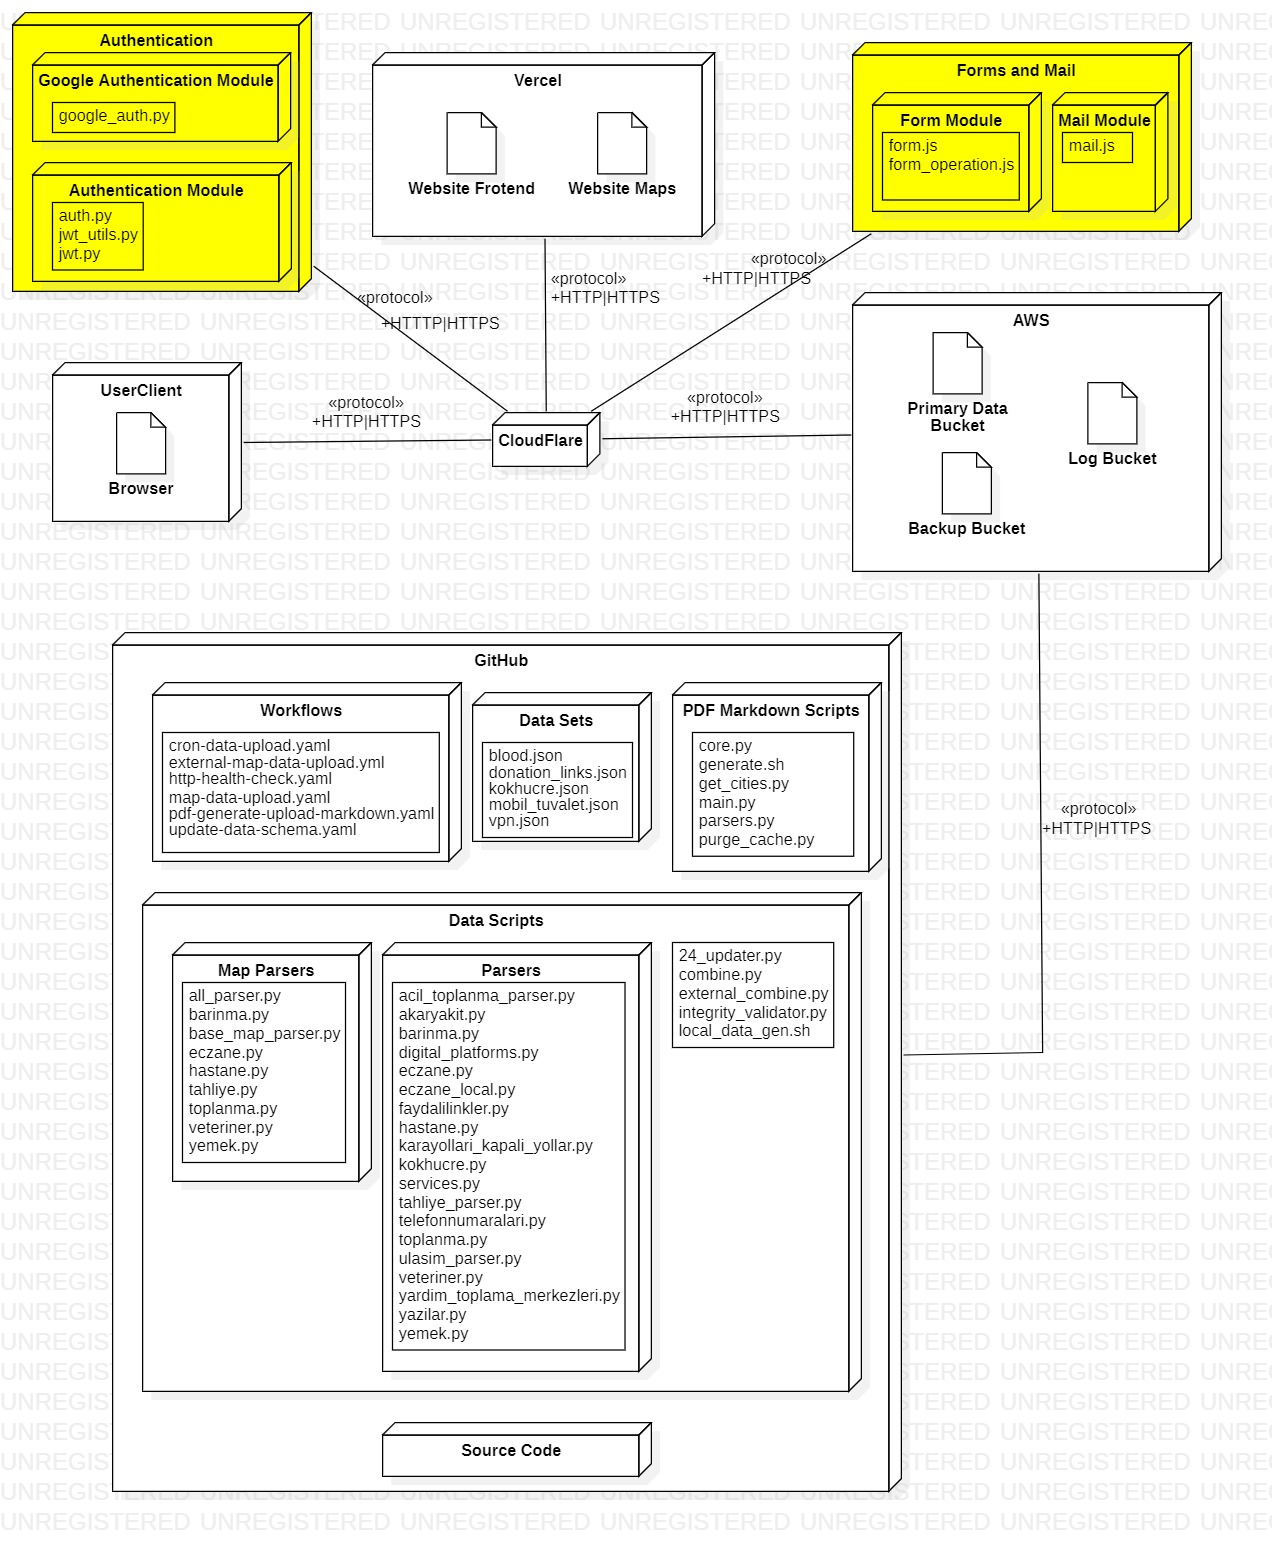
\includegraphics[width=\linewidth]{img/deployment-diagram-s5.jpg}
  \caption{Suggested Deployment Diagram}
\end{figure}

\begin{itemize}
  \item Authentication provides authorized users to register and login. It uses two systems which are Google Authentication and built-in Authentication System.
  \subitem Google Authentication access the Google API for authentication. Built-in authentication system use stored database information with JSON Web Tokens (JWT) for token based authentication system.
  \item Form provides user to send feedback about website and data. Forms to provide feedbacks are defined according to needs. Some operations such as uploading image as well as the basic form operations such as submitting.
  \item Mail modeule sends mails if there is an update in the website.
\end{itemize}

\subsection{Design Rationale}

The entire \afetbilgi\ website system is based on the fundamental principle and primary objective of being an open-source, verified non-profit website. Its purpose is to provide quick information to victims and volunteers without requiring user registration or unnecessary time expenditure. The website is designed with simple buttons and hierarchical routing to relevant datasheets based on user needs. All the different views, including the context, functional, information, and deployment views, are built upon this foundation. In summary, we have proposed enhancements to increase the website's security and dynamism.

In the context view, the diagram explains the basic setup of the \afetbilgi\ website for use by victims and volunteers. The external interface diagram demonstrates how data validators utilize external services like Google Datasheets to retrieve recent data, and AWS to incorporate data from latest.json. Site maintainers and developers also employ Github Actions' CI/CD workflows to continuously update the website and regularly check its data integrity from the AWS S3 bucket where it is hosted. DNS assignments are managed by Cloudflare. Additionally, we have added authentication using Google API as a reliable third-party user registration mechanism. A module for handling mail subscriptions has also been embedded to inform users about potential alerts related to ongoing earthquake emergencies. Similar interfaces are further elaborated in the added components of the external diagram.

In the functional view, we observe the interaction of internal interfaces within a modern modular setup based on object programming principles of interfaces and extensions. The computation components involve regular website health checks using Github workflow actions on Ubuntu environments, with data backups and the last recorded website health saved to AWS buckets. On the internal interface side, modularized entities like TreeNode interfaces ensure proper addition of new data pages and validate their typing according to node descriptions specified. Although the website is static and each data node (having its own webpage on \afetbilgi) does not directly interact with other interfaces, the sequence diagrams effectively demonstrate the process of adding and conforming new data (hot/cold) to node specifications, with workflows assimilating and eventually uploading them to AWS as latest.json files (type-checked and saved via schema.json). Additional components such as Google authentication are handled through external API requests for user registration, and there are internal components for managing mail subscriptions to registered users. Similar new internal interfaces handle these aspects and interact with the additional external components.

The Information View reinforces the project's concept of being stand-alone, with no backend databases or areas for uploading private information such as user details or credit card information. The main stakeholders who appreciate this section are the site data validators and maintainers. The Database Class diagram illustrates the transmission and exchange of variables within interfaces. Although there are no explicit SQL classes or tables, some form of validation and role assignment is required for users to be allowed to update data on the website. All tables and datasheets have common elements like City, Source, Location, and Map components. The CRUD operations table provides a basic summary of the available data-altering options based on the Database Class Diagram, without delving into excessive technical details. Furthermore, an essential user database class has been added, along with additional mail subscription classes, to further formalize and secure the website. Based on the assigned roles, users have authorization to make changes to the website.

Lastly, the Deployment View explains the project repository and its modular nature, with clearly outlined files. This view highlights the project's dependencies on other external entities for data upload and interaction, such as AWS bucket components and exchanging latest.json files with them, along with type conformations defined in schema.json. Parser Python files are executed through external Github Actions' Ubuntu server to fetch and assimilate hot data sheets from relevant Google Datasheets, while cold sheets (manually added data) are simply copied and merged. Finally, the static website will now have some level of dynamism such as a new interface(with a relevant js file in the react project) to generate forms for users to enter feedback after they have logged in/registered via the proper authentication webpage(also new).


\end{document}
